\chapter{Software}
\par Este componente de software tendrá el propósito de asistir al fabricante de cerveza en las tareas de monitoreo, planificación y visualización de datos históricos de experimentos de maceración.

\par En los siguientes incisos, serán descriptas las consideraciones tomadas para la elección de una plataforma sobre la cual se desarrollará la aplicación de Software.

\section{Análisis de alternativas}
    \subsection{Tecnologías}
        \par A continuación se presenta una breve reseña de las plataformas actualmente más relevantes para dispositivos móviles.
        
        \subsubsection{Android}
            \par Android es un sistema operativo, el cual fue inicialmente desarrollado por Android Inc., empresa que Google respaldó económicamente y más tarde, en 2005, compró. Fue diseñado principalmente para dispositivos móviles con pantalla táctil desarrollados por Google o por terceros, como teléfonos inteligentes, tabletas y también, relojes inteligentes, televisores y automóviles. 
            
            \par Android es un sistema operativo basado en el núcleo Linux.
            
        \subsubsection{iOS}
            \par iOS es un sistema operativo móvil de la multinacional Apple Inc. Originalmente desarrollado para el iPhone (iPhone OS), después utilizado en dispositivos como el iPod touch y el iPad. No permite la instalación de iOS en hardware de terceros.
            
            \par iOS se deriva de macOS, que a su vez está basado en Darwin BSD, y por lo tanto es un sistema operativo Tipo Unix.
            
    \subsection{Comparación}
        \par El desarrollo será realizado para una plataforma móvil, de las cuales se tendrán en cuenta las siguientes consideraciones: cantidad de usuarios que la utilicen; tamaño de la comunidad a disposición para dar soporte; disponibilidad de mejores herramientas y utilidades para el desarrollo de aplicaciones.
        
        \par A continuación, se presenta una tabla comparativa en la cual se abordan aspectos de interés para la elección y un análisis concluyente.
        
        \begin{table}[h]
            \centering
            \begin{tabularx}{\textwidth}{|X|X|X|}
                 \hline
                 \multicolumn{3}{|c|}{Tabla comparativa de tecnologías de software}\\
                 \hline
                 Criterios de comparación & Android & iOS \\
                 \hline
                 \hline
                 
                 Porcentaje Mercado (Arg) & 75\% & 19\%  \\
                 \hline
                 
                 Porcentaje Mercado Internacional & 85\% & 14,7\% \\
                 \hline
                 
                 Comunidad de desarrolladores & Muy grande & Amplia pero acorde al número de usuarios\\
                 \hline
                 
                  Entornos desarrollo Propia & Android Studio & Xcode\\
                 \hline
                 
                 Lenguaje de desarrollo & Java, C, C++ y Kotlin & Swift, C, C++ y objective-C\\
                 \hline
                 
                 Familia del SO & Linux & Unix - BSD\\
                 \hline
                 
                 Complejidad de desarrollo & Muy diversa variedad de dispositivos y de versiones del SO & Variedad reducida de dispositivos, versiones de SO comunes a la mayoría\\
                 \hline
                 
                 Entorno & Open Source & Entorno cerrado \\
                 \hline
                 
                 Requerimientos para publicación de aplicación & Ninguna & Debe cumplir requisitos de Apple\\
                 \hline
                 
            \end{tabularx}
            \caption{Comparación de plataformas móviles}
            \label{tab:ComparacionPlataformasMoviles}
        \end{table}

    
    \subsection{Elección}
    \par
    La elección fue realizada a partir de los criterios antes mencionados aplicados sobre la tabla comparativa.
    \par
    Se decidió desarrollar la aplicación para la plataforma \textbf{Android}, considerado, el porcentaje de uso en Argentina, el tamaño de la comunidad de desarrolladores, la gran disponibilidad de herramientas y la sencillez relativa en cuanto a  requerimientos para la publicación de aplicaciones.




\section{Diseño}
    \subsection{Diseño de la interfaz de usuario}
        \par Las figuras \ref{fig:MockUpMainActivity}, \ref{fig:MockUpPlanningActivity}, \ref{fig:MockUpExperimentActivity}, \ref{fig:MockUpInfoMash}, \ref{fig:MockUpCurrentExperienceFragment}, \ref{fig:MockUpStageFragment}, \ref{fig:MockUpGeneralFragment} y \ref{fig:MockUpExperimentFragment} ubicadas en el Anexo, diagraman y describen el diseño y las funcionalidades de la interfaz de usuario (UI) bosquejadas para la aplicación móvil.
        
    \subsection{Diagrama de Clases}
    \par
    En el anexo, Figura 9, puede encontrar el diseño diagrama de clases  un diagrama de clases  de la aplicación.
    
    \subsection{Base de Datos}
        \par En el siguiente diagrama (Figura \ref{fig:DiagramaBdApp}) se esquematiza la base de datos a alojar en la aplicación. En el diagrama se pueden distinguir las tablas a utilizar para la abstracción de la aplicación y el conjunto de relaciones establecidas entre ellas.
        
        \begin{figure}[h]
            \centering
            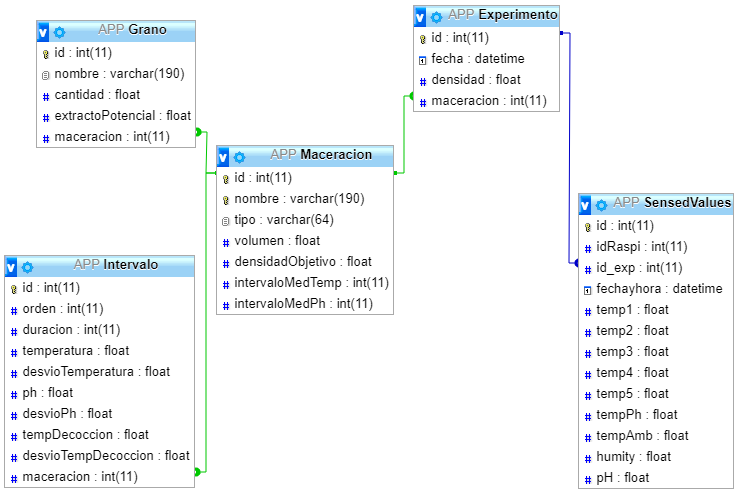
\includegraphics[scale=0.8]{DiagramaBaseDeDatosAPP.jpg}
            \caption{Diagrama de Base de Datos de la aplicación}
            \label{fig:DiagramaBdApp}
        \end{figure}

\section{Implementación}
    \par Esta sección contiene la presentación de los resultados obtenidos del desarrollo de este componente. Como se introdujo anteriormente en el diseño, la arquitectura de una aplicación Android se divide en ciertos elementos denominados \textit{Activities}, los cuales incluyen componentes de interfaz gráfica denominados Vistas(\textit{Views}) y los eventos correspondientes a la interacción con los mismos (patrón \textit{observer}).
    
    \par Debido a la imposibilidad de la desagregación de ciertas funciones, los \textit{activities} incluyen métodos o llamadas que interaccionan con librerías o clases complementarias. Dentro de estas últimos se encuentran el modelo de clases, la interacción con la base de datos y llamadas a las API's, entre otras.
    
    \par Para cada uno de los \textit{activities} de la misma se adjunta la correspondiente descripción general, las funciones que cumple, interacción con clases o librerías complementarias y el modo de uso. 
    
    
        \subsection{Pantalla principal}
            \subsubsection{Descripción}
                \par Es la pantalla con la que inicia la aplicación.
            \subsubsection{Funciones}
            \subsubsection{Modo de uso}